
\documentclass[nooutcomes]{ximera}
%\documentclass[space,handout,nooutcomes]{ximera}

% For preamble materials

\usepackage{pgf,tikz}
\usepackage{mathrsfs}
\usetikzlibrary{arrows}
\usepackage{framed}
\usepackage{amsmath}
%\pgfplotsset{compat=1.16}

\graphicspath{
  {./}
  {algorithms/}
  {../algorithms/}
}

\pdfOnly{\renewenvironment{image}[1][]{\begin{center}}{\end{center}}}

%%% This set of code is all of our user defined commands
\newcommand{\bysame}{\mbox{\rule{3em}{.4pt}}\,}
\newcommand{\N}{\mathbb N}
\newcommand{\C}{\mathbb C}
\newcommand{\W}{\mathbb W}
\newcommand{\Z}{\mathbb Z}
\newcommand{\Q}{\mathbb Q}
\newcommand{\R}{\mathbb R}
\newcommand{\A}{\mathbb A}
\newcommand{\D}{\mathcal D}
\newcommand{\F}{\mathcal F}
\newcommand{\ph}{\varphi}
\newcommand{\ep}{\varepsilon}
\newcommand{\aph}{\alpha}
\newcommand{\QM}{\begin{center}{\huge\textbf{?}}\end{center}}

\renewcommand{\le}{\leqslant}
\renewcommand{\ge}{\geqslant}
\renewcommand{\a}{\wedge}
\renewcommand{\v}{\vee}
\renewcommand{\l}{\ell}
\newcommand{\mat}{\mathsf}
\renewcommand{\vec}{\mathbf}
\renewcommand{\subset}{\subseteq}
\renewcommand{\supset}{\supseteq}
\renewcommand{\emptyset}{\varnothing}
\newcommand{\xto}{\xrightarrow}
\renewcommand{\qedsymbol}{$\blacksquare$}
\newcommand{\bibname}{References and Further Reading}
\renewcommand{\bar}{\protect\overline}
\renewcommand{\hat}{\protect\widehat}
\renewcommand{\tilde}{\widetilde}
\newcommand{\tri}{\triangle}
\newcommand{\minipad}{\vspace{1ex}}
\newcommand{\leftexp}[2]{{\vphantom{#2}}^{#1}{#2}}

%% More user defined commands
\renewcommand{\epsilon}{\varepsilon}
\renewcommand{\theta}{\vartheta} %% only for kmath
\renewcommand{\l}{\ell}
\renewcommand{\d}{\, d}
\newcommand{\ddx}{\frac{d}{dx}}
\newcommand{\dydx}{\frac{dy}{dx}}


\usepackage{bigstrut}


\newenvironment{sectionOutcomes}{}{}

\usepackage{array}
%\setlength{\extrarowheight}{-.2cm}   % Commented out by Findell to fix table headings.  Was this for typesetting division?  
\newdimen\digitwidth
\settowidth\digitwidth{9}
\def~{\hspace{\digitwidth}}
\def\divrule#1#2{
\noalign{\moveright#1\digitwidth
\vbox{\hrule width#2\digitwidth}}}


\title{Algorithms}
\author{Bart Snapp and Brad Findell}
\begin{document}
\begin{abstract}
More problems about algorithms. 
\end{abstract}
\maketitle

%\fixnote{Add a problem about the doubling/halving base-two multiplication algorithm....   Perhaps also include the Mysterious base-two game, or make it an activity.}

\begin{problem}Here is an example of a standard addition algorithm:
\begin{image}
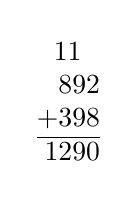
\begin{tikzpicture}
\node at (0,0) {$
\begin{array}{@{}r@{}}
11~~\\
892\\
+398\\ \hline
1290
\end{array}
$};
\end{tikzpicture}
\end{image}
\begin{enumerate}
\item Describe how to perform this algorithm.
\item Provide an additional relevant and revealing example
  demonstrating that you understand the algorithm.
\item Show the ``behind-the-scenes'' algebra that is going on here.
\end{enumerate}
\end{problem} 

\begin{problem}Here is an example of the column addition
  algorithm:\index{addition algorithm!column}
\begin{image}
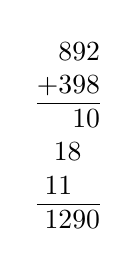
\begin{tikzpicture}
\node at (0,0) {$
\begin{array}{@{}r@{}}
892\\
+398\\ \hline
10\\
18~~\\
11~~~\\ \hline
1290
\end{array}
$};
\end{tikzpicture}
\end{image}
\begin{enumerate}
\item Describe how to perform this algorithm.
\item Provide an additional relevant and revealing example
  demonstrating that you understand the algorithm.
\item Show the ``behind-the-scenes'' algebra that is going on here.
\end{enumerate}
\end{problem} 

\begin{problem}If you check out Problems~\ref{P:MS} and \ref{P:DS}, you will
  learn about ``partial'' algorithms.
\begin{enumerate}
\item Develop a ``partial'' algorithm for addition, give it a name, and describe how to
  perform this algorithm.
\item Provide a relevant and revealing example demonstrating that you
  understand the algorithm.
\item Show the ``behind-the-scenes'' algebra that is going on here.
\end{enumerate}
\end{problem} 

\begin{problem}Here is an example of the banker's addition
  algorithm:\index{addition algorithm!banker's}
\begin{image}
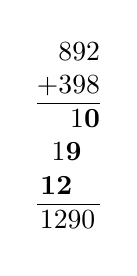
\begin{tikzpicture}
\node at (0,0) {$
\begin{array}{@{}r@{}}
892\\
+398\\ \hline
1\textbf{0}\\
1\textbf{9}~~\\
\textbf{12}~~~\\ \hline
1290\,
\end{array}
$};
\end{tikzpicture}
\end{image}
\begin{enumerate}
\item Describe how to perform this algorithm.
\item Provide an additional relevant and revealing example
  demonstrating that you understand the algorithm.
\item Show the ``behind-the-scenes'' algebra that is going on here.
\end{enumerate}
\end{problem} 

\begin{problem}Here is an example of a standard subtraction
  algorithm:\index{subtraction algorithm!standard}
\begin{image}
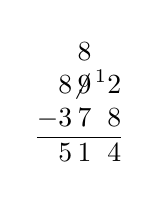
\begin{tikzpicture}
\node at (0,0) {
$\begin{array}{@{}r@{}r@{}r@{}r@{}}
&   & 8 &  \\
& 8 & \not{\hspace{-.2ex}9} & \hspace{.3ex}\leftexp{1}2\\
- & 3 & 7 & 8\\ \hline
& 5 & 1 & 4
\end{array}$
};
\end{tikzpicture}
\end{image}
\begin{enumerate}
\item Describe how to perform this algorithm.
\item Provide an additional relevant and revealing example
  demonstrating that you understand the algorithm.
\item Show the ``behind-the-scenes'' algebra that is going on here.
\end{enumerate}
\end{problem} 

\begin{problem}Here is an example of the subtraction by addition
  algorithm:\index{subtraction algorithm!by addition}
\begin{image}
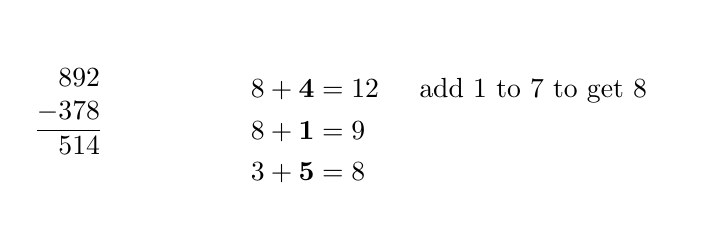
\begin{tikzpicture}
\node at (0,0) {$
\begin{array}[c]{@{}r@{}}
892\\
-378\\ \hline
514
\end{array} 
\qquad\leftrightsquigarrow\qquad
\begin{minipage}{40ex}
\begin{align*}
8 + \textbf{4} &= 12 & &\text{add $1$ to $7$ to get $8$} \\
8 + \textbf{1} &= 9 \\
3 + \textbf{5} &= 8
\end{align*}
\end{minipage}
$};
\end{tikzpicture}
\end{image}
\begin{enumerate}
\item Describe how to perform this algorithm.
\item Provide an additional relevant and revealing example
  demonstrating that you understand the algorithm.
\item Show the ``behind-the-scenes'' algebra that is going on here.
\end{enumerate}
\end{problem} 

\begin{problem}Here is an example of the Austrian subtraction
  algorithm:\index{subtraction algorithm!Austrian}
\begin{image}
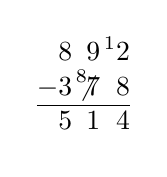
\begin{tikzpicture}
\node at (0,0) {$
\begin{array}{@{}r@{}r@{}r@{}r@{}}
& 8 & 9 & \hspace{.3ex}\leftexp{1}2\\
- & 3 & \hspace{.3ex}\leftexp{8}{\hspace{-.8ex}\not{\hspace{0ex}7}} & 8\\ \hline
& 5 & 1 & 4
\end{array}
$};
\end{tikzpicture}
\end{image}
\begin{enumerate}
\item Describe how to perform this algorithm.
\item Provide an additional relevant and revealing example
  demonstrating that you understand the algorithm.
\item Show the ``behind-the-scenes'' algebra that is going on here.
\end{enumerate}
\end{problem} 

\begin{problem}If you check out Problems~\ref{P:MS} and \ref{P:DS}, you will
  learn about ``partial'' algorithms.
\begin{enumerate}
\item Develop a ``partial'' algorithm for subtraction, give it a name, and describe how to
  perform this algorithm.
\item Provide a relevant and revealing example demonstrating that you
  understand the algorithm.
\item Show the ``behind-the-scenes'' algebra that is going on here.
\end{enumerate}
\end{problem} 

\begin{problem}Here is an example of a standard multiplication algorithm:
\begin{image}
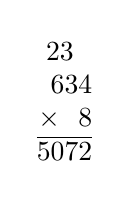
\begin{tikzpicture}
\node at (0,0) {$
\begin{array}{@{}r@{}}
23~~\\
634\\
\times~~8\\ \hline
5072
\end{array}
$};
\end{tikzpicture}
\end{image}

\begin{enumerate}
\item Describe how to perform this algorithm.
\item Provide an additional relevant and revealing example
  demonstrating that you understand the algorithm.
\item Show the ``behind-the-scenes'' algebra that is going on here.
\end{enumerate}
\end{problem} 

\begin{problem}\label{P:MS} Here is an example of the partial-products 
  algorithm: \index{multiplication algorithm!partial-products}\index{partial products algorithm}
\begin{image}
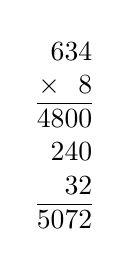
\begin{tikzpicture}
\node at (0,0) {$
\begin{array}{@{}r@{}}
634\\
\times~~8\\ \hline
4800\\
240\\
32\\ \hline
5072
\end{array}
$};
\end{tikzpicture}
\end{image}
\begin{enumerate}
\item Describe how to perform this algorithm.
\item Provide an additional relevant and revealing example
  demonstrating that you understand the algorithm.
\item Show the ``behind-the-scenes'' algebra that is going on here.
\end{enumerate}
\end{problem} 

\begin{problem}Here is an example of a standard division algorithm:
\begin{image}
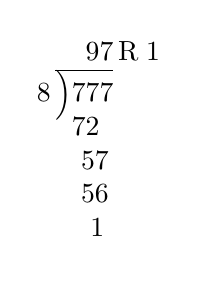
\begin{tikzpicture}
\node at (0,0) {$
8\,\begin{array}[b]{@{}r@{}r} 
97 &\, \text{R}\;1\\ 
\cline{1-1}
\Big)\begin{array}[t]{@{}l@{}} 777\\ 
72 \\ 
\divrule{0}{2}  ~57 \\
 ~56\\
 \divrule{1}{2}
~~1
\end{array}
\end{array}
$};
\end{tikzpicture}
\end{image}
\begin{enumerate}
\item Describe how to perform this algorithm.
\item Provide an additional relevant and revealing example
  demonstrating that you understand the algorithm.
\item Show the ``behind-the-scenes'' algebra that is going on here.
\end{enumerate}
\end{problem} 

\begin{problem}\label{P:DS} Here is an example of the partial quotients
  algorithm:\index{division algorithm!partial-quotients}
\begin{image}
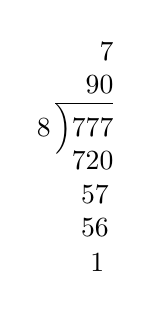
\begin{tikzpicture}
\node at (0,0) {$
8\,\begin{array}[b]{@{}r@{}} 
7 \\
90\\ 
\hline
\Big)\begin{array}[t]{@{}l@{}} 777\\ 
720 \\ 
\divrule{0}{3}  
~57 \\
 ~56\\
 \divrule{1}{2}
~~1
\end{array}
\end{array}
$};
\end{tikzpicture}
\end{image}
\begin{enumerate}
\item Describe how to perform this algorithm.
\item Provide an additional relevant and revealing example
  demonstrating that you understand the algorithm.
\item Show the ``behind-the-scenes'' algebra that is going on here.
\end{enumerate}
\end{problem} 

\begin{problem}Here is another example of the partial-quotients division
  algorithm:\index{division algorithm!partial-quotients}
\begin{image}
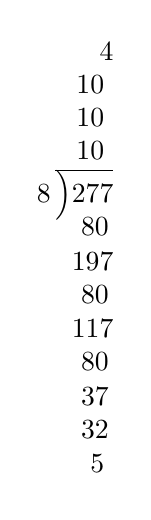
\begin{tikzpicture}
\node at (0,0) {$
8\,\begin{array}[b]{@{}r@{}} 
4\\
10~\\
10~\\
10~\\ 
\hline
\Big)\begin{array}[t]{@{}l@{}} 277\\ 
~80 \\ 
\divrule{0}{3}  
197 \\
~80 \\
\divrule{0}{3}
117 \\
~80 \\
\divrule{0}{3}
~37 \\
~32 \\
\divrule{1}{2}
~~5
\end{array}
\end{array}
$};
\end{tikzpicture}
\end{image}
\begin{enumerate}
\item Describe how to perform this algorithm---be sure to explain how
  this is different from the scaffolding division algorithm.
\item Provide an additional relevant and revealing example
  demonstrating that you understand the algorithm.
\item Show the ``behind-the-scenes'' algebra that is going on here.
\end{enumerate}
\end{problem} 

\begin{problem}Here is an example of a standard multiplication
  algorithm:\index{multiplication algorithm!standard}
\begin{image}
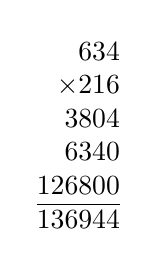
\begin{tikzpicture}
\node at (0,0) {$
\begin{array}{@{}r@{}}
634\\
\times 216\\ \divrule{1}{5}
3804 \\
6340 \\
126800\\ \hline
136944
\end{array}
$};
\end{tikzpicture}
\end{image}
\begin{enumerate}
\item Describe how to perform this algorithm.
\item Provide an additional relevant and revealing example
  demonstrating that you understand the algorithm.
\item Show the ``behind-the-scenes'' algebra that is going on
  here---you may assume that you already know the algebra behind the 
standard multiplication algorithm.
\end{enumerate}
\end{problem} 

\begin{problem}Here is an example of the addition algorithm with decimals:
\begin{image}
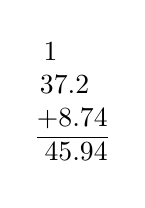
\begin{tikzpicture}
\node at (0,0) {$
\begin{array}{@{}r@{}}
1\hspace*{4.2ex}\\
37.2~~\\
+8.74\\ \hline
45.94
\end{array}
$};
\end{tikzpicture}
\end{image}

\begin{enumerate}
\item Describe how to perform this algorithm.
\item Provide an additional relevant and revealing example
  demonstrating that you understand the algorithm.
\item Show the ``behind-the-scenes'' algebra that is going on here.
\end{enumerate}
\end{problem} 

\begin{problem}Here is an example of the multiplication algorithm with
  decimals:
\begin{image}
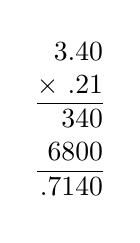
\begin{tikzpicture}
\node at (0,0) {$
\begin{array}{@{}r@{}}
3.40\\
\times~.21\\ \hline
340\\
6800\\
\hline
.7140
\end{array}
$};
\end{tikzpicture}
\end{image}
\begin{enumerate}
\item Describe how to perform this algorithm.
\item Provide an additional relevant and revealing example
  demonstrating that you understand the algorithm.
\item Show the ``behind-the-scenes'' algebra that is going on here.
\end{enumerate}
\end{problem} 

\begin{problem}Here is an example of the division algorithm without remainder:
\begin{image}
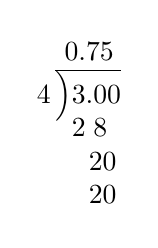
\begin{tikzpicture}
\node at (0,0) {$
4\,\begin{array}[b]{@{}l@{}} 
~0.75\\
\hline
\Big)\begin{array}[t]{@{}l@{}} 3.00\\ 
2\;8 \\ 
\divrule{0}{3}  ~\;20 \\
 ~\;20\\
 \divrule{1}{3} \vspace{-1.4em} \\ 
 \divrule{1}{3}
\end{array}
\end{array}
$};
\end{tikzpicture}
\end{image}
\begin{enumerate}
\item Describe how to perform this algorithm.
\item Provide an additional relevant and revealing example
  demonstrating that you understand the algorithm.
\item Show the ``behind-the-scenes'' algebra that is going on here.
\end{enumerate}
\end{problem} 

\begin{problem}In the following addition problem, every digit has been
  replaced with a letter.
\begin{image}
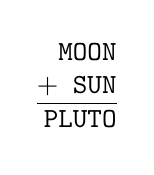
\begin{tikzpicture}
\node at (0,0) {$
\begin{tabular}{@{}r@{}}
\texttt{MOON}\\
$+$\texttt{ SUN}\\ \hline
\texttt{PLUTO}
\end{tabular}
$};
\end{tikzpicture}
\end{image}
Recover the original problem and solution. Explain your reasoning.
Hint: $\texttt{S}=6$ and $\texttt{U}=5$.
\end{problem} 

\begin{problem}In the following addition problem, every digit has been
  replaced with a letter.
\begin{image}
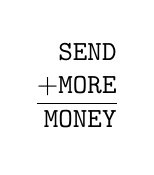
\begin{tikzpicture}
\node at (0,0) {$
\begin{tabular}{@{}r@{}}
\texttt{SEND}\\
$+$\texttt{MORE}\\ \hline
\texttt{MONEY}
\end{tabular}
$};
\end{tikzpicture}
\end{image}

Recover the original problem and solution. Explain your reasoning.
\end{problem} 

\begin{problem}In the following subtraction problem, every digit has been
  replaced with a letter.
\begin{image}
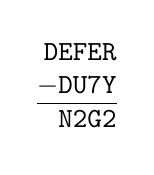
\begin{tikzpicture}
\node at (0,0) {$
\begin{tabular}{@{}r@{}}
\texttt{DEFER}\\
$-$\texttt{DU7Y}\\ \hline
\texttt{N2G2}
\end{tabular}
$};
\end{tikzpicture}
\end{image}
Recover the original problem and solution. Explain your reasoning.
\end{problem} \begin{problem}In the following two subtraction problems, every digit has been
  replaced with a letter.
\begin{image}
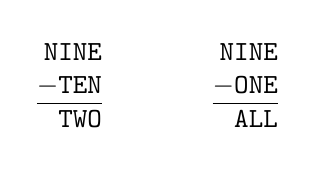
\begin{tikzpicture}
\node at (0,0) {$
\begin{tabular}{@{}r@{}}
\texttt{NINE}\\
$-$\texttt{TEN}\\ \hline
\texttt{TWO}
\end{tabular}
\qquad\qquad
\begin{tabular}{@{}r@{}}
\texttt{NINE}\\
$-$\texttt{ONE}\\ \hline
\texttt{ALL}
\end{tabular}
$};
\end{tikzpicture}
\end{image}
Using both problems simultaneously, recover the original problems and
solutions. Explain your reasoning.
\end{problem} 

\begin{problem}In the following multiplication problem, every digit has been
  replaced with a letter.
\begin{image}
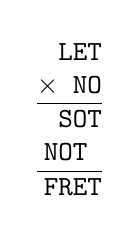
\begin{tikzpicture}
\node at (0,0) {$
\begin{tabular}{@{}r@{}}
\texttt{LET}\\
$\times$\texttt{ NO}\\ \hline
\texttt{SOT}\\
\texttt{NOT$~$}\\
\hline
\texttt{FRET}
\end{tabular}
$};
\end{tikzpicture}
\end{image}
Recover the original problem and solution. Explain your reasoning.

%% \begin{teachingnote}
%% The next two problems may seem tedious, but they are very rewarding
%% for students when they are able to finally solve them. While the
%% student should be encouraged to use a calculator, the solution is not
%% pure ``guess and check'' and there is a lot of reasoning that goes
%% into the solution.
%% \end{teachingnote}

\end{problem} 

\begin{problem}The following is a long division problem where every digit
  except 7 was replaced by X.
\settowidth\digitwidth{X}
\def~{\hspace{\digitwidth}}
\begin{image}
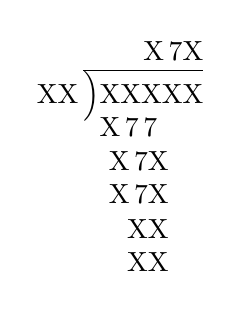
\begin{tikzpicture}
\node at (0,0) {$
\text{XX}\,\begin{tabular}[b]{@{}r@{}}
X\,7X \\ \hline
\Big)\begin{tabular}[t]{@{}l@{}}
XXXXX \\
X\,7\,7 \\ \divrule{0}{3}
~X\,7X \\
~X\,7X \\ \divrule{1}{3}
~~~XX\\ 
~~~XX \\ \divrule{3}{2}\vspace{-1.4em} \\ 
 \divrule{3}{2}
\end{tabular}
\end{tabular}
$};
\end{tikzpicture}
\end{image}
Recover the digits from this long division problem. Explain your
reasoning.
%% \begin{teachingnote}
%% Remind students to use their calculator and that to start,
%% $\mathrm{XX}\cdot \mathrm{X} = \mathrm{X}77$.
%% \end{teachingnote}

\end{problem}
 
\begin{problem}The following is a long division problem where the various digits were
replaced by X except for a single $8$. The double bar indicates that the remainder is 0.

\begin{image}
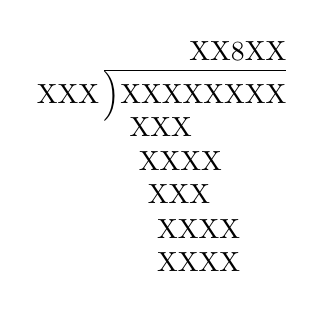
\begin{tikzpicture}
\node at (0,0) {$
\text{XXX}\,\begin{tabular}[b]{@{}r@{}}
XX8XX \\ \hline
\Big)\begin{tabular}[t]{@{}l@{}}
XXXXXXXX \\
~XXX \\ \divrule{1}{3}
~~XXXX \\
~~~XXX \\ \divrule{3}{3}
~~~~XXXX\\ 
~~~~XXXX \\ \divrule{4}{4}\vspace{-1.4em} \\ 
 \divrule{4}{4}
\end{tabular}
\end{tabular}
$};
\end{tikzpicture}
\end{image}

Recover the digits from this long division problem. Explain your
reasoning.

\end{problem}



\end{document}